\documentclass[oneside]{article}
\usepackage{fullpage}
\usepackage[pdftex]{graphicx}
\DeclareGraphicsExtensions{.png,.pdf}
\graphicspath{{images/}}
\usepackage{hyperref}
\usepackage{verbatim}
\usepackage[format=plain,font=small]{caption}
\usepackage[small]{titlesec}
\usepackage[round,sectionbib]{natbib}
\bibliographystyle{plainnat}
\renewcommand\rmdefault{bch}
\linespread{1.07} 

\begin{document}

\title{Glyph-maps for visualising climate data and models}
\author{Cook, Hofmann, Wickham, Wickham, Cheng}

% Drawing trend lines on map
%   - How to
%   - Comparison to coloring slope
%   - Reference to Grinstein icon plots
% Pickett RM and Grinstein GG (1988). Iconographics 
% displays for visualizing multidimensional data. 
% In Proc. IEEE Conference on Systems, Man, and Cybernetics, pages 514-19.
% Note the later work on metaphoric data display, garbage work!
%   - Alexander Gribov's work http://rosuda.org/software/Gauguin/gauguin.html
%   - Spatial star plots by Andrews http://www.udallas.edu:8080/~andrews/software/software.html
%   - Look at what Bertin does
%
% Interactive graphics
% Data processing
%
% Perhaps the GHCN data? Not gridded
% NOAA data, almost grid, but over ocean, so maps more tricky
% NARCAP from NCAR?
% Fill in with NASA data, to start, try to put new data for final version
\maketitle

\section{Introduction}

Need a colourful map, facetted by year \& month

Simple, but effective, technique that combines aspects of glyphs, facetted plots and map-charts. Particularly well suited for the type of temporal-spatial data, commonly seen in climate.

Glyph-maps have attributes of both glyphs (stars, faces, profiles, ...), inviting exploration at the global level, and small-multiple time series, allowing local exploration of individual series. Allow to see both geographic context and individual locations simultaneously.

An interesting attribute of these glyph plots is that the position of graphical elements is determined by major and minor axes. For maps, the major axes are latitude and longitude, and the minor axes are typically time on the x-axis and some measurement or model prediction on the y-axis.

Avoids one problem that plagues glyph displays: the ordering of the variables. Although some techniques exist to ameliorate this problem \citep{kleiner:1981,hurley:2010}, they are not necessary with time data because it is intrinsically ordered.

These displays tend to be particularly effective when printed in large format, as the much higher resolution of print (600 dpi) compared to computer  screen (72-120 dpi) allows for much finer reading. These are high-density data displays in the best tradition of Tufte. Wall size maps are not usually practical during analysis, but are very engaging.

Will first explore for regularly gridded data, a simple starting point and a common output of climate models, and then show a few simple extensions to deal with non-rectangular grids and irregular locations, as exemplified by raw climate data which is typically collect at irregular locations.

\section{Generating a time series at each location}

A big advantage of glyph-maps is that they can be generated with existing graphics software, after a simple pre-processing step. This makes them immediately accessible to a wide audience. The graphics in this paper were created in R \citep{R} using ggplot2 \citep{me:ggplot2,wickham:2007d} and \citep{me:plyr}, but are readily implemented in any statistical programming environment.  Code and data is available in the online supplementary materials.

Because the x and y locations are linear combinations of two variables, these types of displays can also be built interactively by software that supports tours, such as DataViewer, XGobi or GGobi.  This technique is used to good effect in \citet{buja:1996a}.

\section{Reference lines}

Space-time-glyphs often require reference lines: it is difficult to compare the relative location of glyphs in different regions. As noted by \citet{cleveland:1993a}, a \emph{visual reference grid} is important for accurate perception of values, particularly of important properties of lines like slope and minima. This is illustrated well by the previous plot of monthly coefficients. When we add a reference to each location, Figure~\ref{fig:ref-basic}, it becomes much more clear that not only is there a difference in shape between the Northern and Southern hemispheres, but there is also a location shift: values in the North are much higher than values in the South. It is difficult to see this without reference lines.

Figure~\ref{fig:ref-basic} shows two variants of a reference, a line drawn at the overall mid-range, and a box drawn around each grid cell. We prefer using white for such references because it is minimally perceptible: you can see it easily if you concentrate on it, but it does not otherwise distract from the perception of the graphic. Note the careful choice of layering: the map is drawn under mid-range lines, but over boxes.

\begin{figure}[htbp]
  \centering
  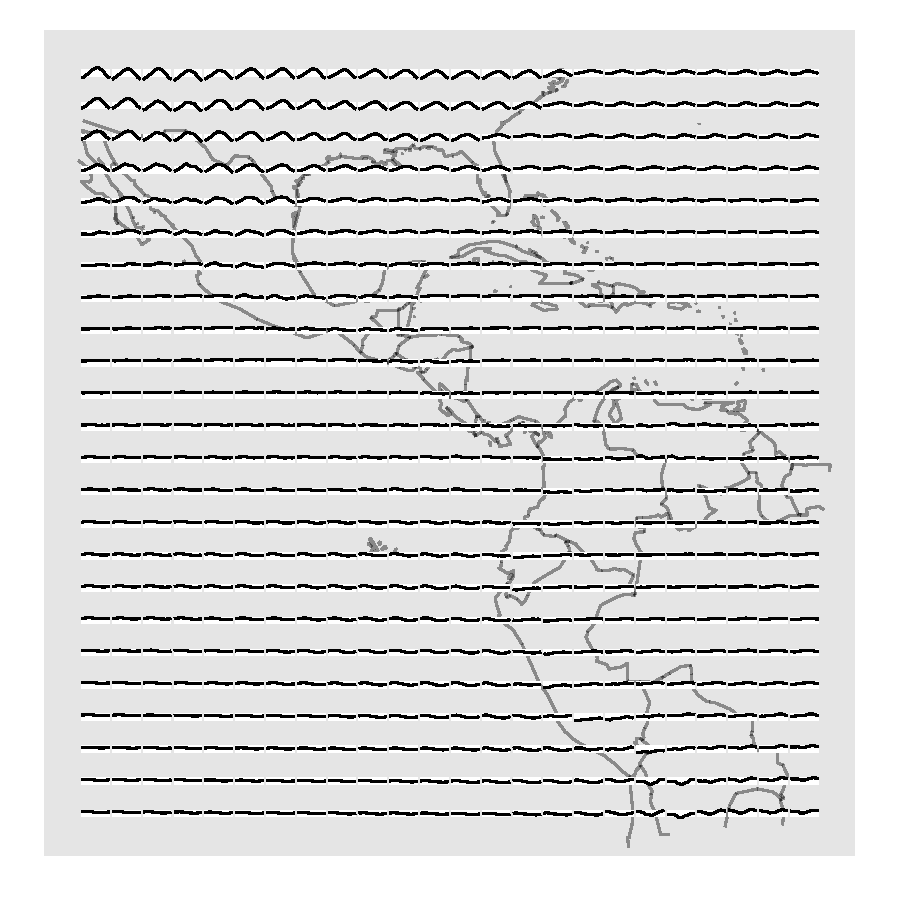
\includegraphics[width=0.5\linewidth]{ref-line}%
  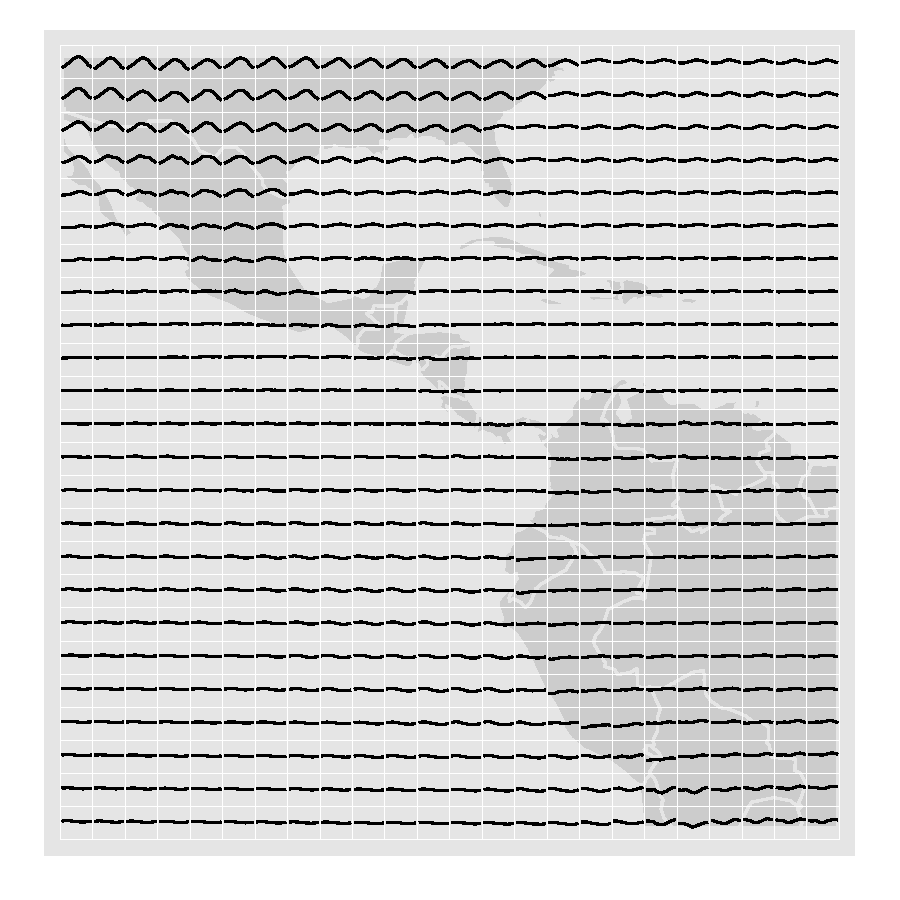
\includegraphics[width=0.5\linewidth]{ref-box}
  \caption{caption}
  \label{fig:ref-basic}
\end{figure}

Other types of reference information can also be usefully added. 
Other ways of display additional data:

\begin{itemize}

  \item Map variable to colour or transparency of line. 
  
  \item Colour of reference lines/boxes.
  
  \item Highlight special points in an additional layer.

  \item Fill colour of reference boxes. 
  
\end{itemize}

A particularly useful application of this technique is when display model predictions to also display some measure of model fit, so that appropriate care can be taken to avoid over-interpreting predictions from models that did not fit well.

Figure~\ref{fig:ref-adv} shows two applications of these ideas, adding the month with the highest average temperature in either the foreground or background. Careful colour choice is necessary so that this information is perceptible, but not distracting.

\begin{figure}[htbp]
  \centering
    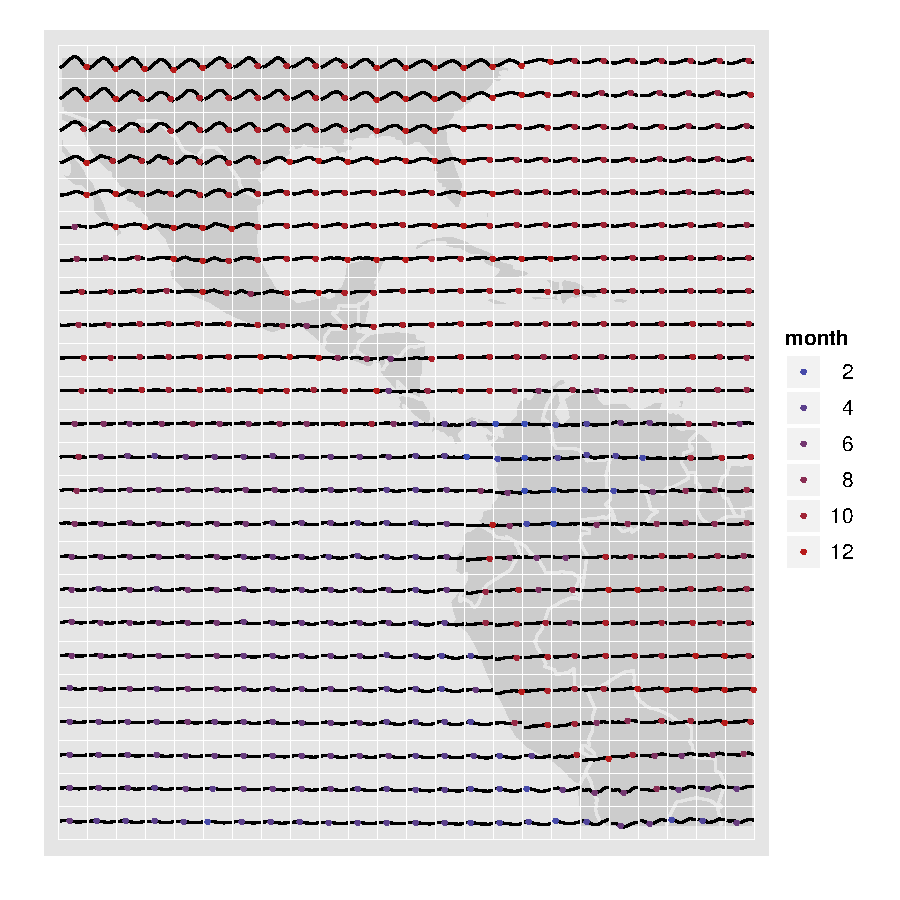
\includegraphics[width=0.5\linewidth]{ref-max-1}%
    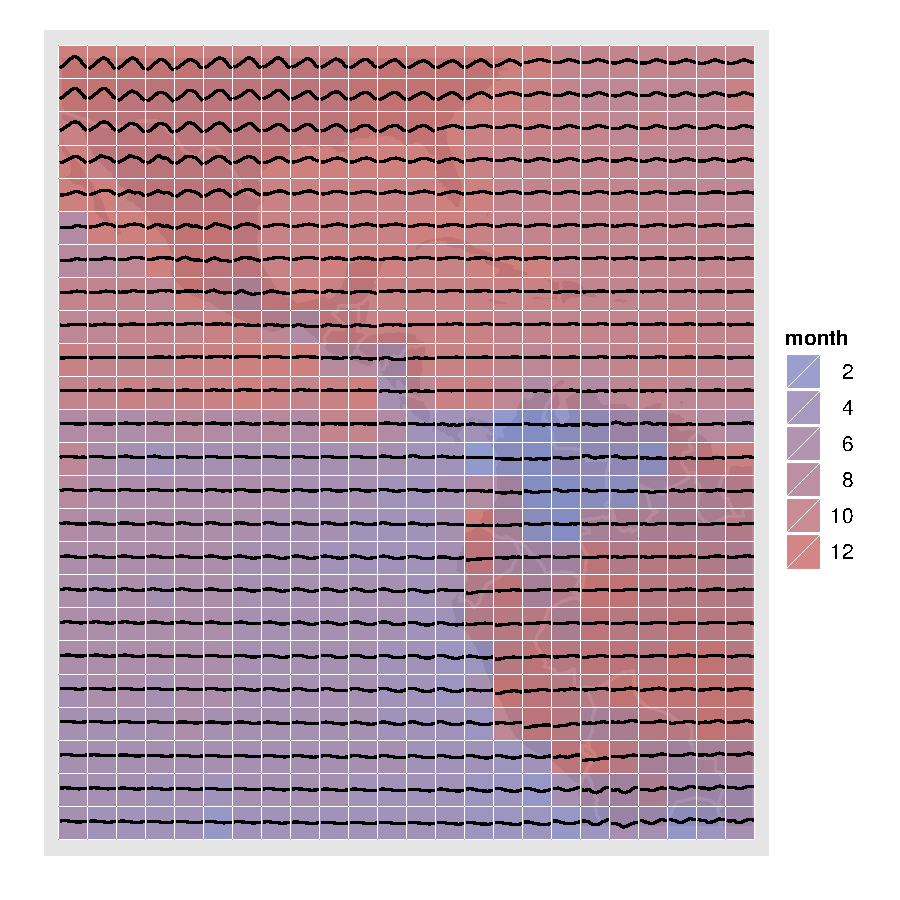
\includegraphics[width=0.5\linewidth]{ref-max-2}
  \caption{caption}
  \label{fig:ref-adv}
\end{figure}


\section{Radial icons/star glyphs}

These time series glyphs can be readily altered to support circular variables, by projecting each line into polar coordinates and joining the ends. This type of display is best suited for variables that are truly circular, such as seasonal patterns or angles (such as for wind direction).

Cite star glyphs.

The alteration to the data transformation is quite simple. Without loss of generality, we assume that $y_{minor}$ becomes $r$, the radius, and $x_{minor}$ becomes $theta$ the angle, both rescaled to lie between 0 and 1. Then the glyph $x$ coordinate is given by $x_{major} + \frac{w \cdot r}{2} \cos(2 \pi \theta)$, and the $y$ coordinate by $y_{major} + \frac{h \cdot r}{2} \sin(2 \pi \theta)$.

\begin{figure}[htbp]
  \centering
  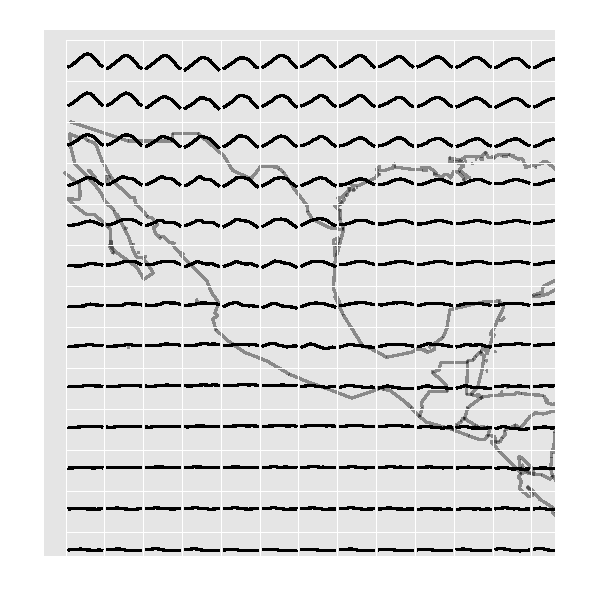
\includegraphics[width=2in]{month-cartesian}
  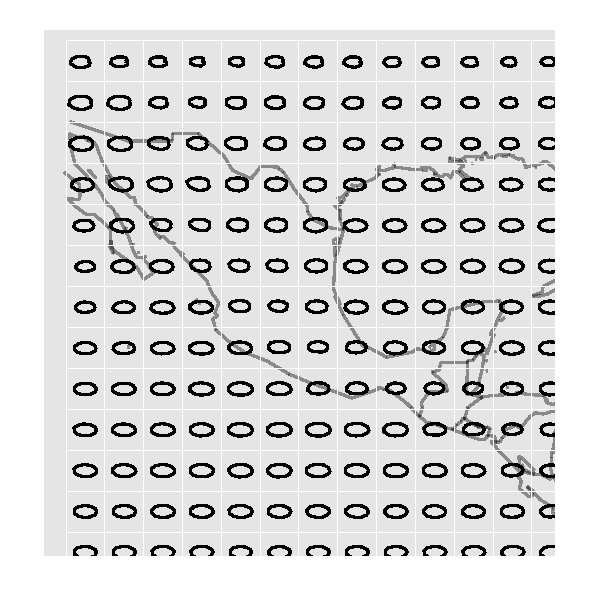
\includegraphics[width=2in]{month-polar}
    
  \caption{Monthly averages in (left) Cartesian coordinates and (right) polar coordinates.}
  
  \label{fig:cycle}
\end{figure}

\section{Scatterplots}

So far we have limited ourselves to always mapping some aspect of time on the x-axis. But the method is much more general. Figure~\ref{fig:cloud} shows how by mapping another variable to the x-axis, in this case low-cloud level on x and high-cloud level on y, we can explore how this 2d distribution varies over space. Again, summarising the data with models is very useful: the second plot displays a loess curve fit to the data instead of the individual points.  

\begin{figure}[htbp]
  \centering
    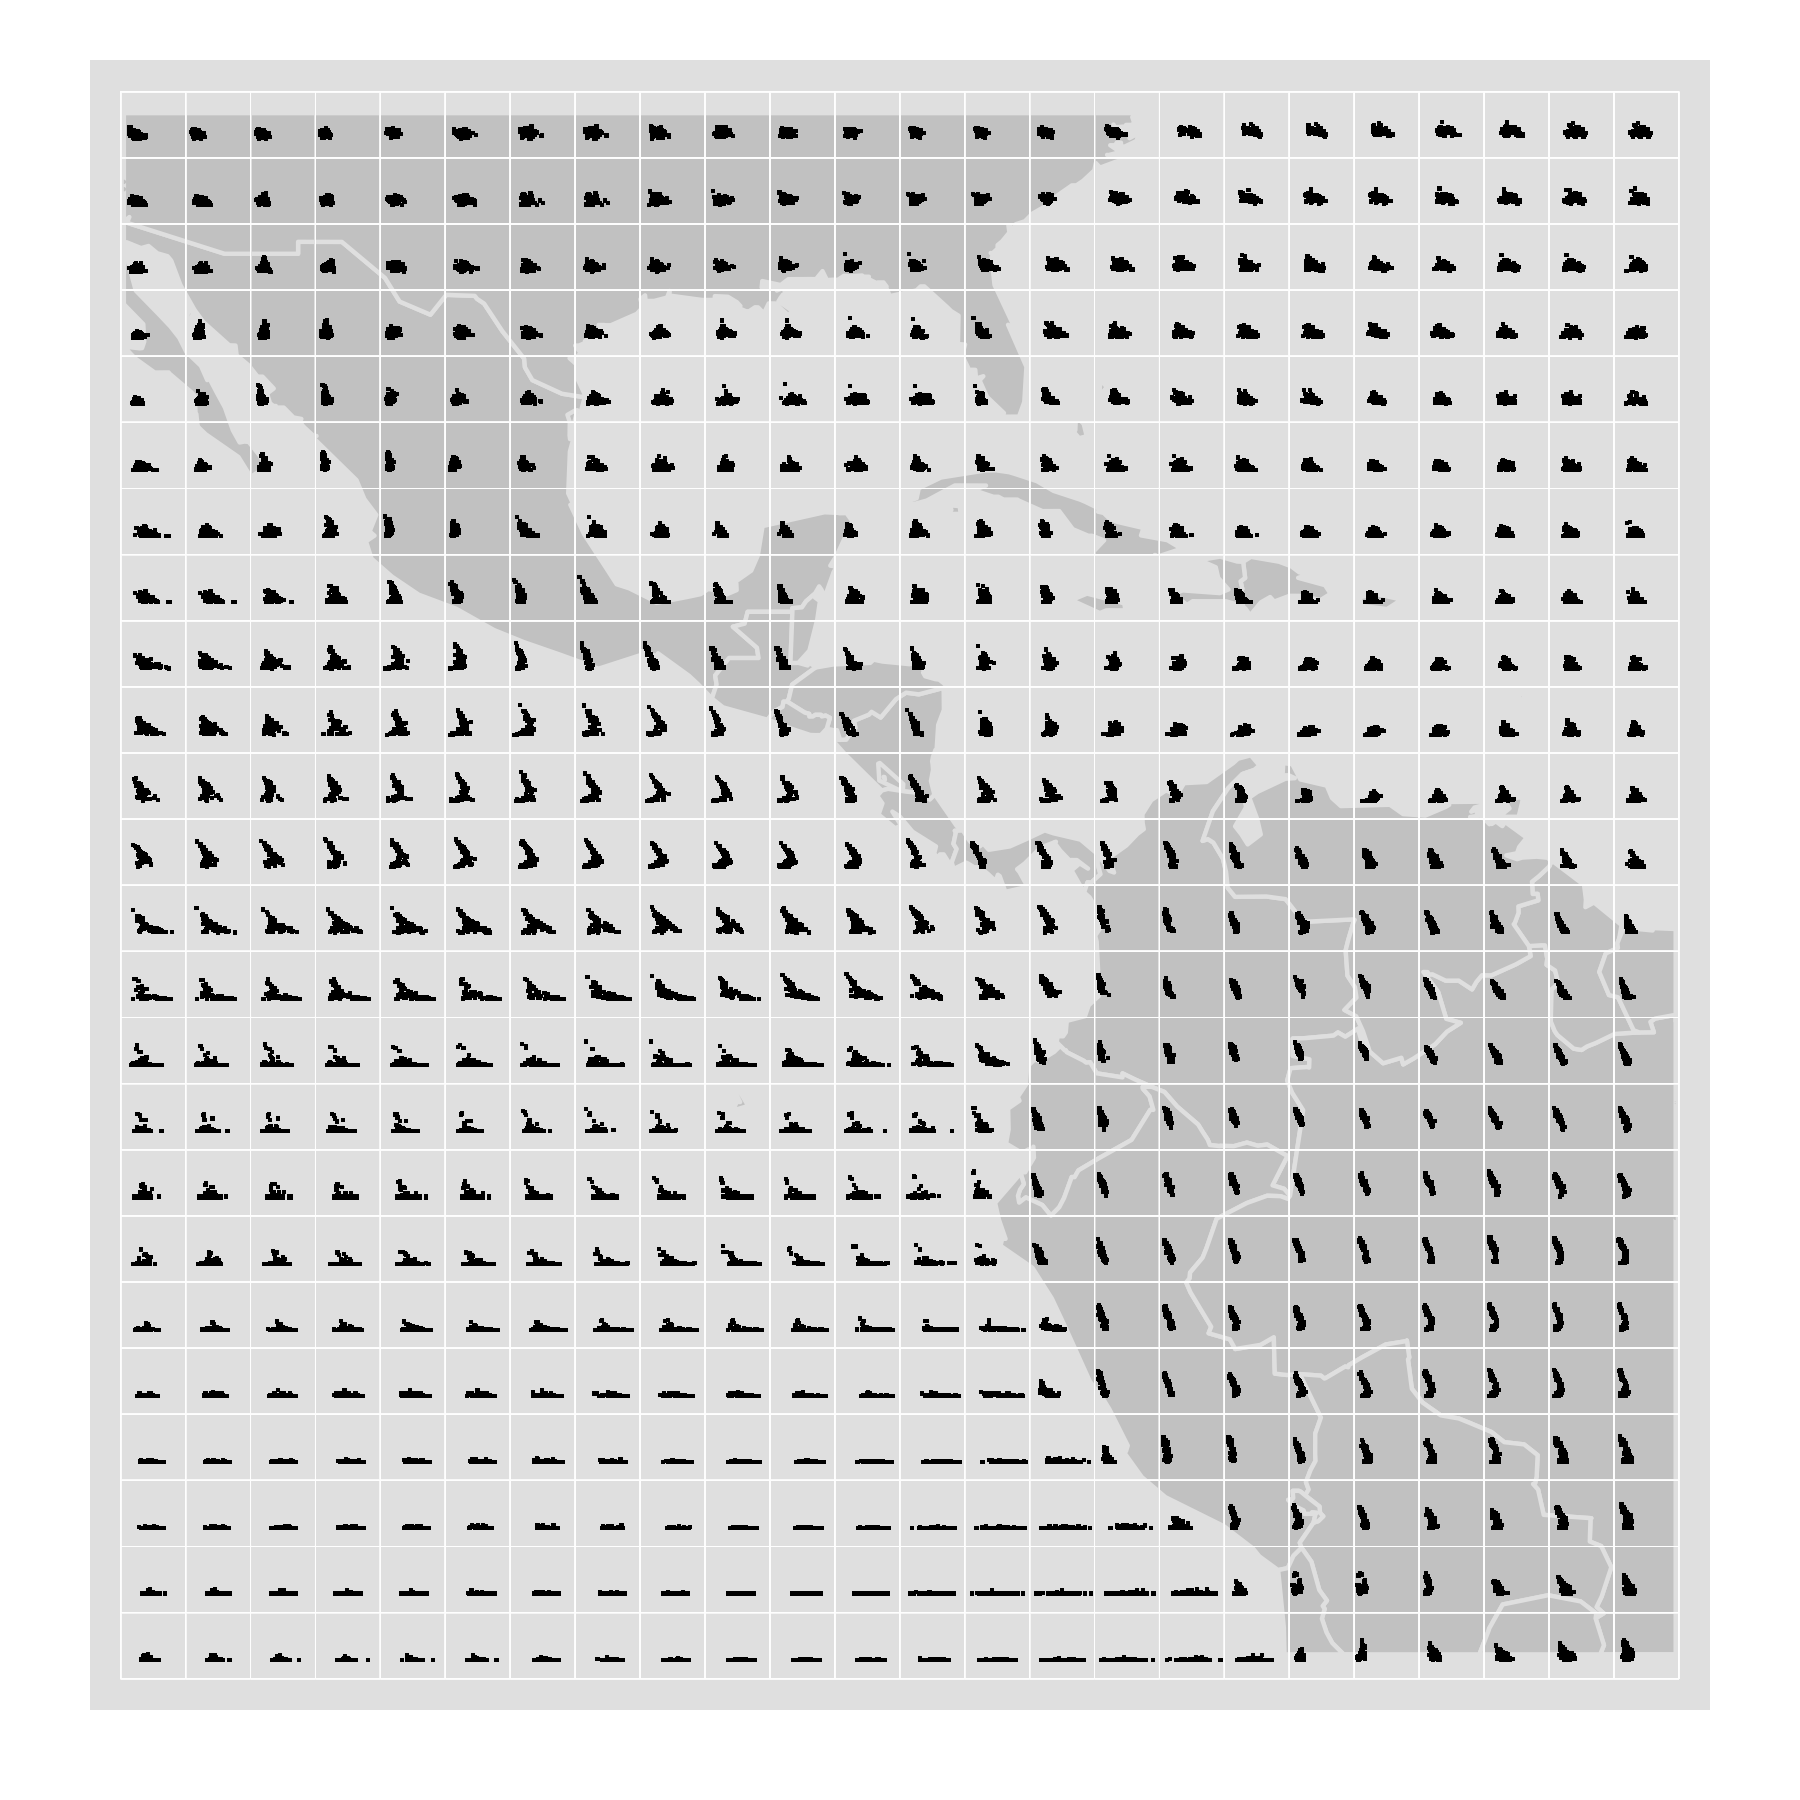
\includegraphics[width=0.5\linewidth]{clouds}%
    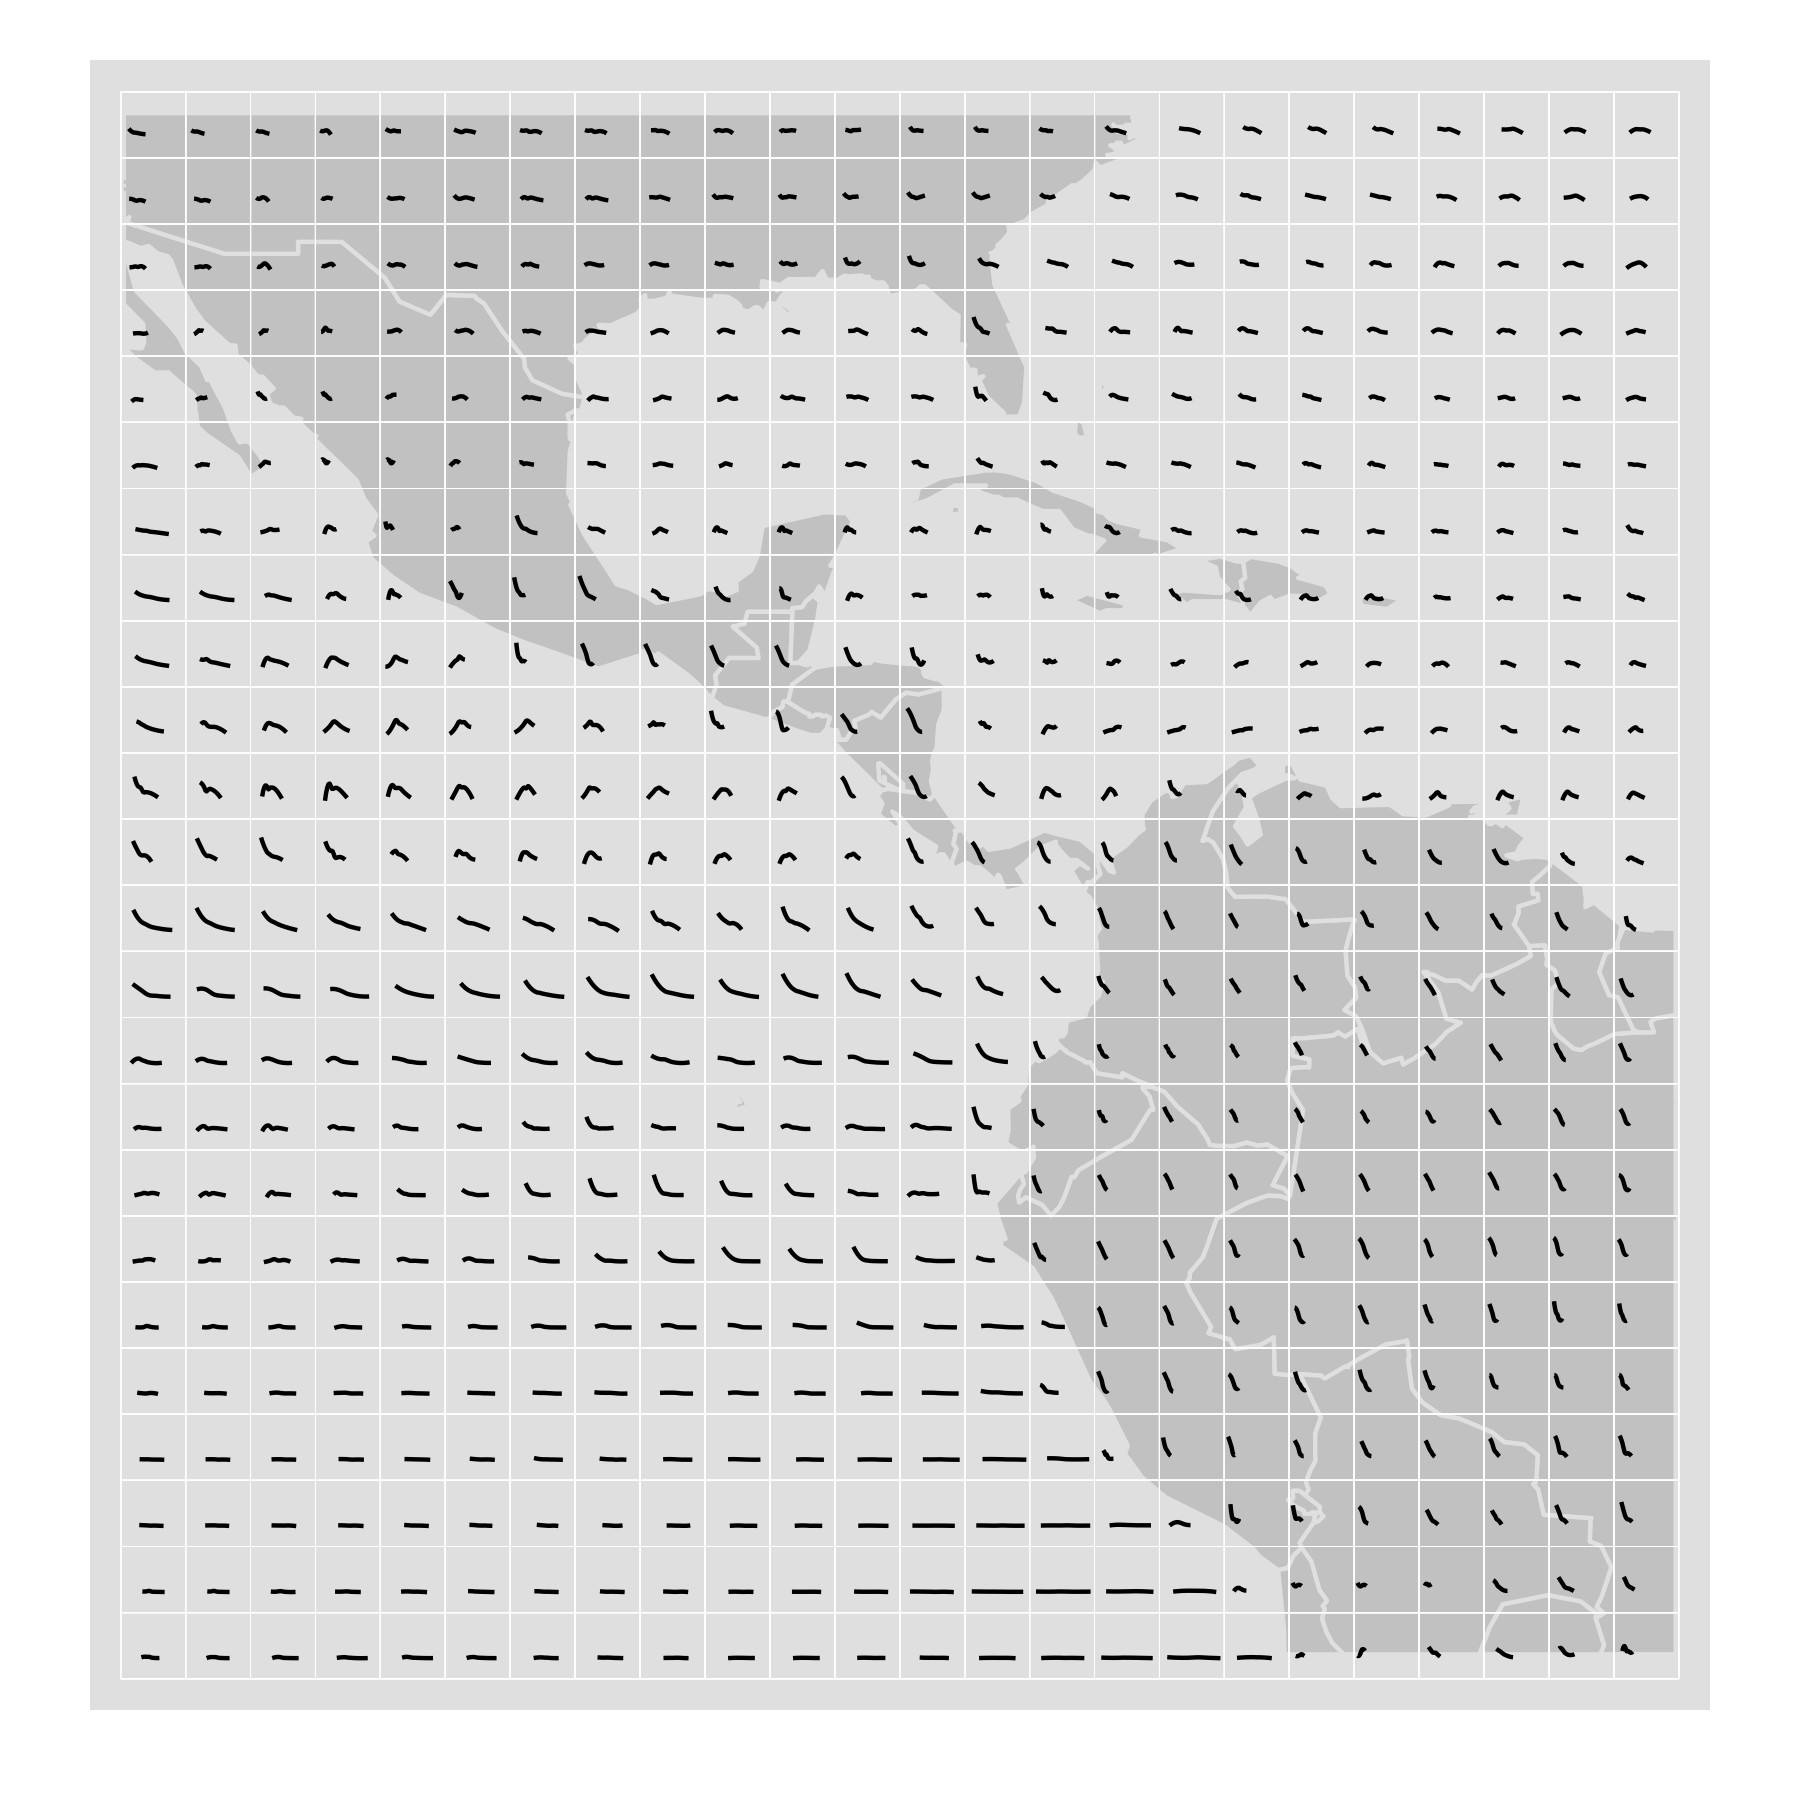
\includegraphics[width=0.5\linewidth]{clouds-smooth}
  \caption{caption}
  \label{fig:cloud}
\end{figure}

\section{Effect of scale}

Partitioning is a extremely useful technique: product plots, ANOVA, ...  For glyph plots, it's often useful to partition the glyphs into shape and scale components, decomposing the values into a product of maximum and scaled values. This is revealing for smooth models of surface temperature.

\begin{figure}[htbp]
  \centering
  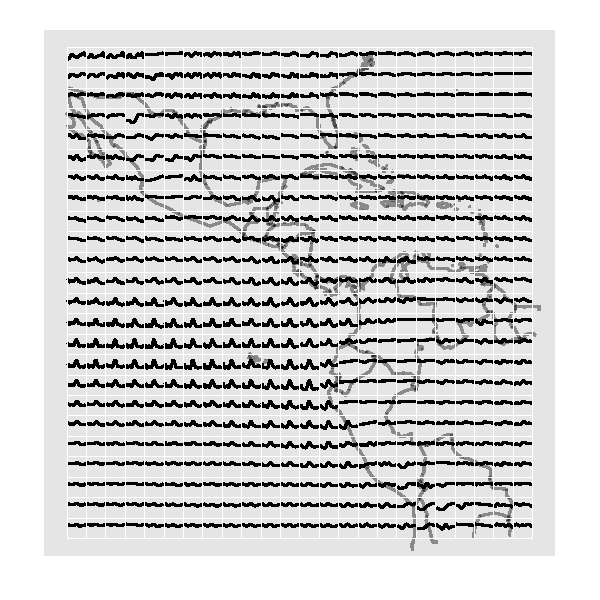
\includegraphics[width=0.5\linewidth]{month-rescale-max}%
  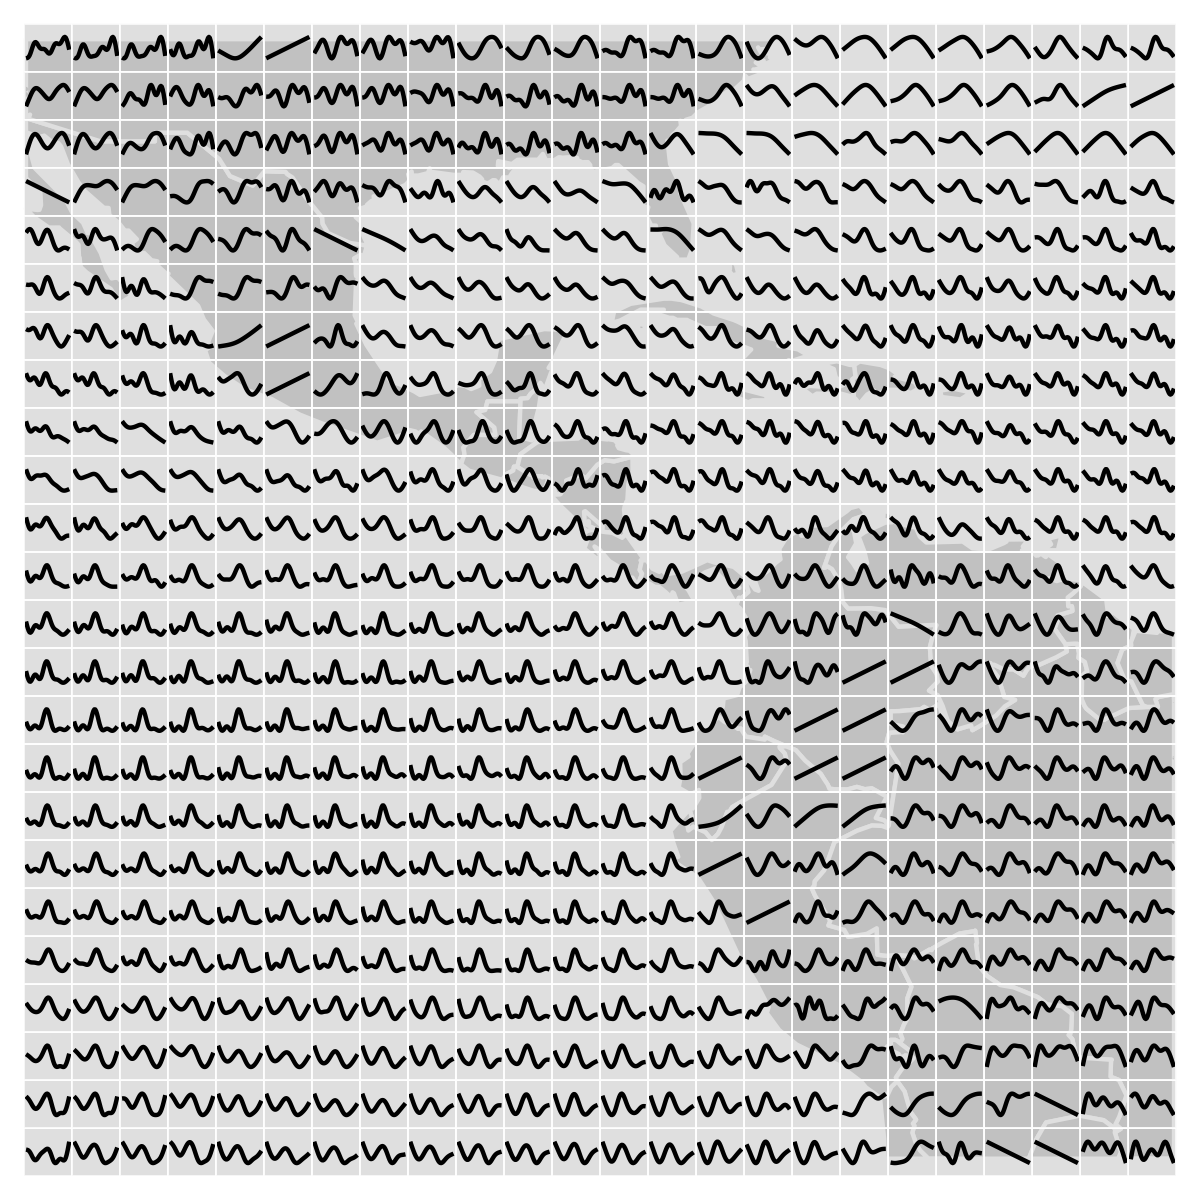
\includegraphics[width=0.5\linewidth]{month-rescale01}
  \caption{caption}
  \label{fig:label}
\end{figure}

Other types of scaling: scale range to 0-1 (subtract min and divide by range), standardise mean and standard deviation (or robust variants). 

Equivalent to using individual scales in facetted graphics.


\section{Regular vs irregular locations}

\subsection{Non-rectangular grids}

Rectangular, but not in this projection.  Other types of regular grids.

\subsection{Irregular locations}

\section{Conclusions}

\bibliography{references}

\end{document}